\documentclass[11pt,a4paper]{article}
\usepackage{natbib}
\usepackage{graphicx}
\usepackage{subcaption}
\usepackage{amsmath}
\usepackage{amsfonts}
\usepackage{enumitem}
\usepackage{setspace}
\usepackage{booktabs}
\usepackage{tabulary}
\usepackage{hyperref}
\usepackage[capitalise,noabbrev]{cleveref}
\usepackage[a4paper, total={6in, 8in}]{geometry}
\usepackage{tikz}
\usetikzlibrary{shapes,arrows,positioning}

\tikzset{
    %Define standard arrow tip
    >=stealth',
    %Define style for boxes
    block/.style={
           rectangle,
           draw=black,
           text width=6.5em,
           minimum height=3em,
           text centered},
    % Define arrow style
    arrow/.style={
           ->,
           thick,
           shorten <=2pt,
           shorten >=2pt,
           }
}

\bibliographystyle{plainnat}
\setcitestyle{authoryear,open={(},close={)}}

\newcommand{\pkg}[1]{{\fontseries{b}\selectfont #1}} 


\title{\textbf{A path model of energy intensity}}
\author{S. Drake Siard}
\date{2020 May 5}
\begin{document}

\maketitle

\begin{abstract}
This project aims to further develop a published path model, originally applied to Bangladesh, to analyse the direct and indirect impacts of growth, industrialization, technological innovation, and trade openness on energy intensity.
The model is first validated by replicating the results in the original paper, and some choices regarding model construction and data treatment are re-assessed.
A modified version of the model then applied to more recent data in India and the UK, where the directions of industrialisation and technological innovation differ, to see if the original hypotheses hold.

Word count: \em{Drake forgot to do this!}
 
\end{abstract}

\tableofcontents

\pagebreak

\section{Introduction}\label{sec:introduction}

Energy intensity, defined as the demand for energy per unit of output, is a critical measure of economic efficiency; it becomes every more important as the world economy develops and world populations continue to rise.
Decreasing energy intensity is a necessary condition for the developing world's economic growth to continue through this century without overwhelming the world's limited resources, and for the developed world to maintain its quality of life while reducing their environmental impact.
A better understanding of the drivers of energy intensity would thus benefit both the developed and developing world.

\cite{panHowIndustrializationTrade2019} cite an extensive literature on energy intensity and its influencing factors, and extract four commonly described determinants of energy intensity: industrialization, trade openness, technological innovation, and economic growth.
These nature of these variables, and the specific economic data series used to represent them, are described in greater detail in \cref{sec:data_sources}.
\cite{panHowIndustrializationTrade2019} also mention a number of models and analyses that attempt to estimate the effect of these variables. 
The authors note that due to the interdependence of these variables there may both direct and indirect effects, and propose four specific hypotheses for the interactions:
\begin{enumerate}[label=\textbf{H.\arabic*}]
\item Industrialisation has positive direct impact on energy intensity.
\item Industrialization has negative indirect impact on energy intensity through technological innovation.
\item Trade openness has negative direct impact on energy intensity.
\item Trade openness has negative indirect impact on energy intensity through economic growth.
\end{enumerate}

\cite{panHowIndustrializationTrade2019} propose a path model (which they describe as novel) to analyse these effects, and apply it to the specific situation of Bangladesh, 1986-2015.
This model is outlined and the results analysed in \cref{sec:original_model}.
The results of the original analysis are (partially) replicated, but some questions are raised regarding the significance of the results and the goodness of fit.

To answer these questions, \cref{sec:data_analysis} then revisits the original data, noting some characteristics that suggest alternative transformations and model specifications.
These updated models are then described and evaluated in \cref{sec:revised_model}, and the results are summarised in \cref{sec:conclusion}.

\clearpage

\section{Data Sources}\label{sec:data_sources}
 
As in \cite{panHowIndustrializationTrade2019}, the dependent variable is energy intensity (denoted EI). The two independent variables are level of industrialization (ISG)\footnote{
The abbreviation is due to the original paper labelling this as ``Industrial Share of Growth"; however, the measure actually used is industrial share of output, not of output growth. 
Similarly, the variable P\_GDP is a measure of output per capita, not growth.
} and trade openness (TO), and the two intermediary variables are economic output (P\_GDP) and technological innovation (TI).
The precise definitions are described in \cref{tab:data_source}, supplementing Table 2 in \cite{panHowIndustrializationTrade2019}.
All data is sampled at an annual frequency.
The specific energy intensity measure in this case is not directly available form the database in those units, but is constructed by taking the primary energy use in kg. of oil equivalent per capita, divided by the (2015, PPP-adjusted) \$US GDP per capita.

\begin{table}[tbp]
\centering
\begin{tabulary}{\textwidth}{l l L} 
 \toprule 
 Abbr. & Name & Description and units \\ [1ex] 
 \midrule 
 EI & Energy intensity & Primary energy use in kg. of oil equivalent per ``current" (2018 or 2019, by vintage) \$US of GDP \\ 
 EIb & Energy intensity (alt.) & Primary energy use in kg. of oil equivalent per (2015, PPP-adjusted) \$US of GDP \\ 
 ISG & Industrialisation & Total industry (mining, construction, utilities) value added as \% of GDP \\
 TO & Trade openness & Total value of imports and exports (goods and services) as \% of GDP \\ 
 TI & Technological innovation & Total number of patent applications (direct and PCT national phase entries) \\ 
 P\_GDP & Economic output & GDP in ``current" (2018 or 2019, by dataset) \$US, divided by mid-year population \\ 
 \bottomrule 
\end{tabulary}
\caption{Variable names and descriptions}
\label{tab:data_source}
\end{table}

For the replication phase, in order to most closely match \cite{panHowIndustrializationTrade2019}, it was necessary\footnote{
ISG was revised in the June 2018 vintage, and the ``current" \$US scaler for P\_GDP was rebased in September 2019.
} to use the April 2018 vintage of the data from the WDI Database Archives, \cite{theworldbankWDIDatabaseArchives2018}.
Additional patent data was retrieved directly from the WIPO Statistics Database via the IP Statistics Data Center, \cite{wipoWIPOStatisticsDatabase2020}, and used to fill in gaps in World Bank data where necessary.

For the updated analysis, data was taken directly from the most recent update of the WDI database, \cite{theworldbankWorldDevelopmentIndicators2019}. In addition, an up-to-date alternate energy intensity measure was added from \cite{enerdataGlobalEnergyStatistical2019} and denoted EIb in the dataset.

In the original paper, the data is truncated to the date range 1986-2015, resulting in the summary statistics in \cref{tab:original_summary_stats}.
Comparing these with the Table 3 of \cite{panHowIndustrializationTrade2019}, there is a close match, but not an exact one.
Of some concern is the mismatch in the number of samples of EI: the per capita primary energy use measure used that has been to construct EI is absent for the year 2015, both in previous vintages and the current version of the upstream database.
While we can use incomplete data to estimate the model, this inevitably results in an additional difference with the original paper.

In the original paper, the model is run on the logarithm of the data, with no further transformations. 
This results the variable correlations in \cref{fig:original_summary_corr}; significant correlations (at the 0.01 level) are denoted with an asterisk.
We can compare these results with Table 4 of \cite{panHowIndustrializationTrade2019}. 
It is unclear in the original whether the correlations are of the raw or log data), but again, in either case, we have a close match but not an exact one.

We defer further analysis of the data to \cref{sec:data_analysis}, and use the log-transformed data in the initial replication.


\begin{table}[tbp]
\centering
\begin{tabular}{lrrrrr}
\toprule
{} &    min &     max &   mean &    std &  count \\
\midrule
ISG   &  20.05 &   28.15 &  24.07 &   2.28 &     30 \\
TO    &  16.69 &   48.11 &  30.56 &   9.98 &     30 \\
TI    &  93.00 &  354.00 & 239.20 &  93.50 &     30 \\
P\_GDP & 227.42 & 1210.16 & 498.83 & 261.51 &     30 \\
EI    &   0.20 &    0.49 &   0.35 &   0.07 &     29 \\
\bottomrule
\end{tabular}
\caption{Original data summary statistics}
\label{tab:original_summary_stats}
\end{table}


\begin{figure}[tbp]
\centering
\begin{subfigure}{0.43\textwidth}
\includegraphics[width=\textwidth]{./plots/BGD_201805_correlations.pdf}
\caption{Untransformed data}
\end{subfigure}%
\begin{subfigure}{0.57\textwidth}
\includegraphics[width=\textwidth]{./plots/BGD_201805_correlations_log.pdf}
\caption{Log data}
\end{subfigure}
\caption{Original data correlations}
\label{fig:original_summary_corr}
\end{figure}

\clearpage

\section{Original Model}\label{sec:original_model}

Path models\footnote{ 
Some of this section is a summary of material in \cite{klinePrinciplesPracticeStructural2016}; the interested reader is directed to the source for more details.
} are a subset of structural equation models that deal only with observed variables (as opposed to hidden, or latent variables), where between the exogenous and final endogenous variables there may be one or more mediating endogenous variables.
In the case of this model, openness to trade and industrialisation are the exogenous variables. 
Openness to trade directly affects energy intensity and economic growth, and economic growth in turn affects energy intensity. 
Industrialisation directly affects  energy intensity and technological innovation, which in turn also affects energy intensity.
This model is represented graphically\footnote{
Following Figure 3 in \cite{panHowIndustrializationTrade2019}, we simplify the diagram by dropping the variance notation.
} in \cref{fig:original_model}. 
The parameter naming convention is preserved from the original: that is, $P_{y,x}$ represents the regression coefficient of an endogenous variable $y$ of an exogenous variable $x$.

\begin{figure}[tbp]
\centering
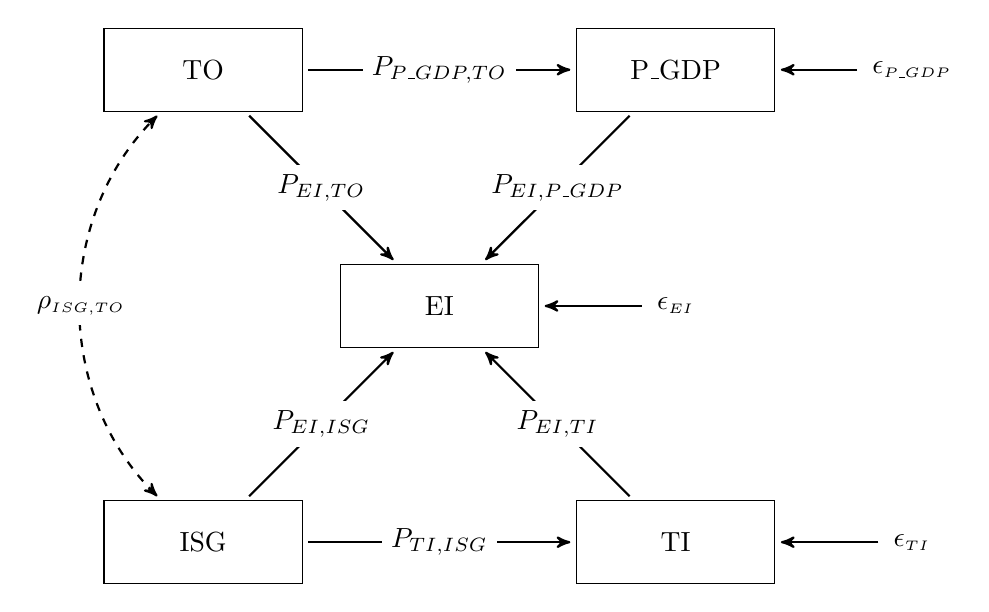
\begin{tikzpicture}[node distance = 3cm, auto]
    \node [block] (EI) {EI};
    \node [above of=EI] (upper dummy) {};    
    \node [below of=EI] (lower dummy) {};    
    \node [block, left of=upper dummy] (TO) {TO};
    \node [block, left of=lower dummy] (ISG) {ISG};
    \node [block, right of=upper dummy] (PGDP) {P\_GDP};
    \node [block, right of=lower dummy] (TI) {TI};
    \node [right of=PGDP] (epsPGDP) {$\epsilon_{\scriptscriptstyle{P\_GDP}}$};
    \node [right of=EI] (epsEI) {$\epsilon_{\scriptscriptstyle{EI}}$};
    \node [right of=TI] (epsTI) {$\epsilon_{\scriptscriptstyle{TI}}$};

	\path[->] (ISG) edge[arrow] node[anchor=center, fill=white] {$P_{EI,ISG}$} (EI);
	\path[->] (ISG) edge[arrow] node[anchor=center, fill=white] {$P_{TI,ISG}$} (TI);
	\path[->] (TO) edge[arrow] node[anchor=center, fill=white] {$P_{EI,TO}$} (EI);
	\path[->] (TO) edge[arrow] node[anchor=center, fill=white] {$P_{P\_GDP,TO}$} (PGDP);
	\path[->] (PGDP) edge[arrow] node[anchor=center, fill=white] {$P_{EI,P\_GDP}$} (EI);
	\path[->] (TI) edge[arrow] node[anchor=center, fill=white] {$P_{EI,TI}$} (EI);
	\path[->] (epsPGDP) edge[arrow] (PGDP);
	\path[->] (epsEI) edge[arrow] (EI);	
	\path[->] (epsTI) edge[arrow] (TI);
	\path (ISG) 
		edge[arrow, <->, bend left=45, dashed] 
		node[anchor=center, fill=white] {$\rho_{\scriptscriptstyle{ISG,TO}}$} 
		(TO);
\end{tikzpicture}
\caption{Path model for EI, mediated by P\_GDP and TI}
\label{fig:original_model}
\end{figure}

Alternatively, we can represent this model as a system of three linear equations:
\begin{align}
TI &= \alpha_{TI} + P_{TI,ISG} TO + \epsilon_{TI} \label{eq:ti}\\
P\_GDP &= \alpha_{P\_GDP} + P_{P\_GDP,TO} TO + \epsilon_{P\_GDP} \label{eq:pgdp}\\
EI &= \alpha_{EI} + P_{EI,ISG} ISG + P_{EI,TO} TO + P_{EI,TI} TI + P_{EI,P\_GDP} P\_GDP + \epsilon_{EI} \label{eq:ei}
\end{align}

This model is recursive; the disturbance processes of the endogenous variables are assumed to be uncorrelated, and all causal effects are strictly unidirectional (there are no feedback loops).
As the model is recursive, it is possible to consistently estimate it using OLS regression, but here we follow \cite{panHowIndustrializationTrade2019} in using maximum likelihood estimation.
It is also over-identified: there are twelve parameters to estimate (three means for the endogenous variables, three variances for the disturbances, and six regression coefficients) and fifteen data points (the sample covariances), leaving three degrees of freedom.
The original paper used SPSS Amos 23; in our case, the model was fitted using an R software package for latent variable modeling called \pkg{lavaan}, \cite{rosseelLavaanPackageStructural2012}, and supplementary analysis was performed using the \pkg{semTools} package, \cite{jorgensenSemToolsUsefulTools2019}.\footnote{
Additional code for generating model predictions and residuals was drawn from user contributions that have not yet been merged with the main \pkg{semTools} codebase.
See \url{https://github.com/simsem/semTools/pull/25} and \url{https://github.com/simsem/semTools/compare/master...drakesiard:residual-predict} for more detail.
}

We this by imputing missing data with a case-wise (full-information) ML estimation, as performed by Amos. 
The complete program output for the model can be found in \cref{sec:program_output}.
The (raw and standardised) coefficient estimates are given in \cref{tab:original_estimates}; we compare these with Table 3 in \cite{panHowIndustrializationTrade2019}, looking at the standardised estimates for the mediating values and unstandardised for the final .
The $R^{2}$ values for the individual endogenous variables are given only for comparison purposes; p-values below 0.01 are marked with an asterisk.
Standard errors are not given in the original, but included here for clarity.

The values for \cref{eq:ti} and \cref{eq:pgdp} match fairly closely, and the significance of the parameters and goodness of fit for \cref{eq:ei} match.

\begin{table}[tbp]
\centering
\begin{tabular}{llllrrrl}
\toprule
Equation & Dep. var. & Ind. var. &      Coefficient &  Est. (std.) &  S.E. (std.) & p-value & $R^{2}$ \\
\midrule
    (1) &        TI &       ISG &     $P_{TI,ISG}$ &        0.800 &        0.055 &       * &   0.641 \\
    (2) &    P\_GDP &        TO &  $P_{P\_GDP,TO}$ &        0.940 &        0.016 &       * &   0.883 \\
    (3) &        EI &       ISG &     $P_{EI,ISG}$ &        0.128 &        0.077 &   0.094 &   0.985 \\
        &        EI &        TO &      $P_{EI,TO}$ &        0.083 &        0.094 &   0.375 &         \\
        &        EI &        TI &      $P_{EI,TI}$ &        0.073 &        0.039 &   0.060 &         \\
        &        EI &    P\_GDP &  $P_{EI,P\_GDP}$ &       -1.230 &        0.062 &       * &         \\
\bottomrule
\end{tabular}
\caption{Original model parameter estimates}
\label{tab:original_estimates}
\end{table}






First, the sample size ($n=29$ or 30) is at the very lower bound of what might be considered acceptable.

Second, the model fit itself is not

Acceptable values for the fit measures are discussed in \cite{klinePrinciplesPracticeStructural2016}; for this analysis, we refer to the values in \cite{parryFitIndicesCommonly2020}.



\section{Data Analysis}\label{sec:data_analysis}

\section{Revised Model}\label{sec:revised_model}

\section{Conclusion}\label{sec:conclusion}
Maybe.

\clearpage

\appendix

\renewcommand{\refname}{\section{References}}.
\bibliography{project}

\clearpage

\section{Appendices}


\subsection{Program Output}\label{sec:program_output}

\newgeometry{margin=2cm}
\pagestyle{empty}

\begin{figure}[htbp]
\begin{subfigure}{\textwidth}
\begin{verbatim}
lavaan 0.6-5 ended normally after 64 iterations

  Estimator                                         ML
  Optimization method                           NLMINB
  Number of free parameters                         12
                                                      
  Number of observations                            30
  Number of missing patterns                         2
                                                      
Model Test User Model:
                                              Standard      Robust
  Test Statistic                                14.849      14.804
  Degrees of freedom                                 3           3
  P-value (Chi-square)                           0.002       0.002
  Scaling correction factor                                  1.003
    for the Yuan-Bentler correction (Mplus variant) 

Model Test Baseline Model:

  Test statistic                               226.218     233.615
  Degrees of freedom                                 9           9
  P-value                                        0.000       0.000
  Scaling correction factor                                  0.968

User Model versus Baseline Model:

  Comparative Fit Index (CFI)                    0.945       0.947
  Tucker-Lewis Index (TLI)                       0.836       0.842
                                                                  
  Robust Comparative Fit Index (CFI)                         0.946
  Robust Tucker-Lewis Index (TLI)                            0.837

Loglikelihood and Information Criteria:

  Loglikelihood user model (H0)                 71.433      71.433
  Scaling correction factor                                  0.882
      for the MLR correction                                      
  Loglikelihood unrestricted model (H1)         78.858      78.858
  Scaling correction factor                                  0.907
      for the MLR correction                                      
                                                                  
  Akaike (AIC)                                -118.866    -118.866
  Bayesian (BIC)                              -102.052    -102.052
  Sample-size adjusted Bayesian (BIC)         -139.414    -139.414

Root Mean Square Error of Approximation:

  RMSEA                                          0.363       0.362
  90 Percent confidence interval - lower         0.193       0.193
  90 Percent confidence interval - upper         0.556       0.555
  P-value RMSEA <= 0.05                          0.003       0.003
                                                                  
  Robust RMSEA                                               0.363
  90 Percent confidence interval - lower                     0.193
  90 Percent confidence interval - upper                     0.556

Standardized Root Mean Square Residual:

  SRMR                                           0.041       0.041
\end{verbatim}

\caption{Model summary}
\end{subfigure}
\caption{Original path model output}
\label{fig:orig_model_output}
\end{figure}

\begin{figure}[htbp]\ContinuedFloat
\begin{subfigure}{\textwidth}
\begin{verbatim}

Parameter Estimates:

  Information                                 Expected
  Information saturated (h1) model          Structured
  Standard errors                             Standard

Regressions:
                   Estimate  Std.Err  z-value  P(>|z|)   Std.lv  Std.all
  EI ~                                                                  
    ISG     (p__s)    0.304    0.180    1.684    0.092    0.304    0.128
    TO   (p_ei_to)    0.054    0.061    0.889    0.374    0.054    0.083
    TI   (p_ei_ti)    0.034    0.018    1.939    0.052    0.034    0.073
    P_GD    (p__p)   -0.623    0.033  -18.756    0.000   -0.623   -1.230
  TI ~                                                                  
    ISG     (p_t_)    3.995    0.555    7.192    0.000    3.995    0.800
  P_GDP ~                                                               
    TO      (p_p_)    1.214    0.082   14.791    0.000    1.214    0.940

Intercepts:
                   Estimate  Std.Err  z-value  P(>|z|)   Std.lv  Std.all
   .EI                1.384    0.410    3.379    0.001    1.384    6.440
   .TI               -7.298    1.762   -4.142    0.000   -7.298  -16.084
   .P_GDP             1.994    0.277    7.211    0.000    1.994    4.703

Variances:
                   Estimate  Std.Err  z-value  P(>|z|)   Std.lv  Std.all
   .EI                0.001    0.000    3.808    0.000    0.001    0.015
   .TI                0.074    0.019    3.808    0.000    0.074    0.359
   .P_GDP             0.021    0.006    3.808    0.000    0.021    0.117

Defined Parameters:
                   Estimate  Std.Err  z-value  P(>|z|)   Std.lv  Std.all
    p_ei_ti_isg       0.137    0.073    1.872    0.061    0.137    0.058
    p_ei_pgdp_to     -0.757    0.065  -11.614    0.000   -0.757   -1.156
    p_ei_isg_total    0.441    0.167    2.643    0.008    0.441    0.187
    p_ei_to_total    -0.703    0.069  -10.219    0.000   -0.703   -1.073

\end{verbatim}

\caption{Parameter estimates}
\end{subfigure}
\caption{Original path model output}
\end{figure}

\restoregeometry{}


\end{document}
